\documentclass[11pt]{article}

\usepackage{latexsym}
\usepackage{amsmath}
\usepackage{amssymb}
\usepackage{amsthm}
\usepackage{graphicx}
\usepackage{listings}
\graphicspath{ {./images/} }
\usepackage{wrapfig}
% \usepackage{pseudocode}
\usepackage{url}
\usepackage[backref, colorlinks=true, citecolor=red, urlcolor=blue, pdfauthor={Prakash Dhimal}]{hyperref}
\usepackage{chngcntr}
% does not reset figure counter.
\counterwithout{figure}{section}


\newcommand{\handout}[5]{
  \noindent
  \begin{center}
  \framebox{
    \vbox{
      \hbox to 5.78in { {\bf } \hfill #2 }
      \vspace{4mm}
      \hbox to 5.78in { {\Large \hfill #5  \hfill} }
      \vspace{2mm}
      \hbox to 5.78in { {\em #3 \hfill #4} }
    }
  }
  \end{center}
  \vspace*{4mm}
}

\newcommand{\lecture}[4]{\handout{#1}{#2}{#3}{#4}{#1}}

\newtheorem{theorem}{Theorem}
\newtheorem{corollary}[theorem]{Corollary}
\newtheorem{lemma}[theorem]{Lemma}
\newtheorem{observation}[theorem]{Observation}
\newtheorem{proposition}[theorem]{Proposition}
\newtheorem{definition}[theorem]{Definition}
\newtheorem{claim}[theorem]{Claim}
\newtheorem{fact}[theorem]{Fact}
\newtheorem{assumption}[theorem]{Assumption}

% 1-inch margins, from fullpage.sty by H.Partl, Version 2, Dec. 15, 1988.
\topmargin 0pt
\advance \topmargin by -\headheight
\advance \topmargin by -\headsep
\textheight 8.9in
\oddsidemargin 0pt
\evensidemargin \oddsidemargin
\marginparwidth 0.5in
\textwidth 6.5in

\parindent 0in
\parskip 1.5ex
%\renewcommand{\baselinestretch}{1.25}

\begin{document}

\lecture{Final Project Report: Visibility of Point Cloud}{Fall 2019}{Prakash Dhimal}{CS 633 Computational Geometry}

\begin{abstract}

Given a point cloud $ P = P_{1},P_{2},P_{3} ... P_{n} $ and a viewpoint $ C $, is it possible to determine all the points visible from $ C $ directly from the point cloud? Katz et al. \cite{Katz07} have shown that this is indeed the case and that this task can be performed without surface reconstruction and normal estimation. This paper investigates and implements an operator called the \textit{Hidden Points Removal} operator described in \cite{Katz07}, which computes only the visible points from a given viewpoint. The operator is simple and it consists of two steps:
\begin{enumerate}
\item Spherical inversion
\item Convex hull construction
\end{enumerate}

\paragraph{}
During Spherical inversion we transform the points to a new domain. Once the spherical inversion is performed, the convex hull of the transformed set of points union C, the viewpoint, is computed. Points that lie on the convex hull are visible from the given viewpoint.

\end{abstract}

\section{Motivation and Introduction}
We formally define a point cloud $ P $ as follows:
\begin{equation}
\label{eq:1}
P = P_{1},P_{2},P_{3} ... P_{n}
\end{equation}

A point cloud is simply a set of data points in space. It is a collection of points that represent a 3D shape or feature, and might contain additional information about each point $ P_{i} $ such as color. Point clouds are most often created by remote sensing and 3D scanning devices such as Light Detection and Ranging (LiDAR). The use of LiDAR and similar 3D scanning devices has been increasing in the past decade. Figure \ref{simple-point-cloud} shows a simple point cloud with Red Green Blue values associated with each point $ P_{i} $.

Determining the visibility of point cloud is an interesting problem in itself. It is also useful in visualizing point clouds, in view-dependent reconstruction and in shadow casting \cite{Katz07}. Determining visibility can lead to a more robust registration of the points from multiple point clouds. This can also provide information about spatial relations and potential obstacles in the line of sight between two points in space, such analyses have been done in estimating the visibility of a landmark, and in finding the optimal location to place a surveillance camera.

\pagebreak
\begin{figure}[h]
	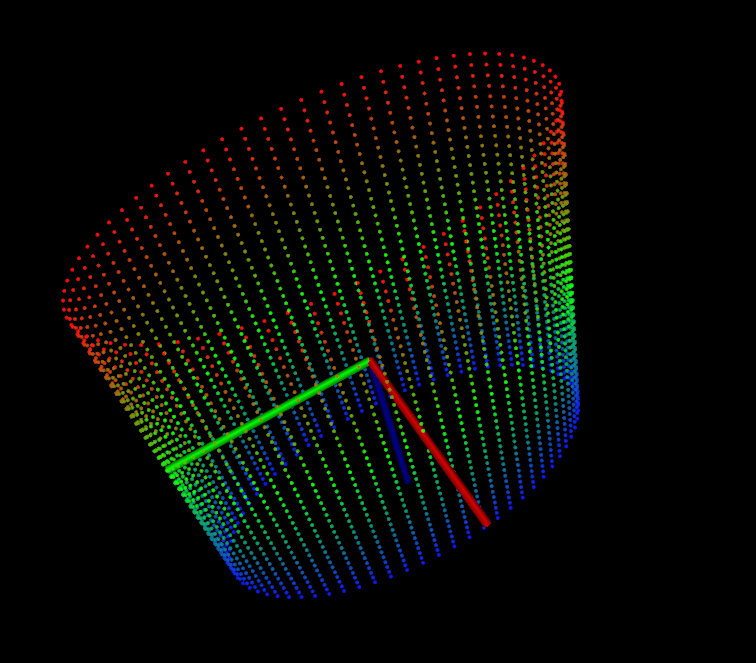
\includegraphics[width=7cm]{simple-pcl}
	\centering
	\caption{Sample Point Cloud}
	\label{simple-point-cloud}
\end{figure}

Suppose that we are given a point cloud depicting an object such as the bunny in figure \ref{fig:bunny-facing-which-way}. If all of the points are visualized, it is difficult to determine whether the bunny is facing forward or backwards. After calculating all of the points visible from a given camera location it can be seen in figure \ref{fig:bunny-facing-front} that the bunny is facing forward.

\begin{figure}[h]
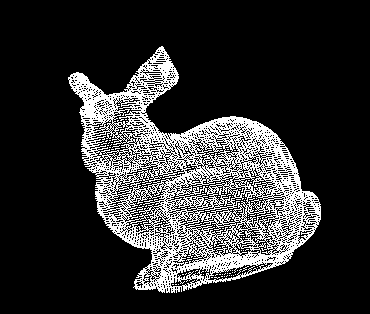
\includegraphics[width=7cm]{bunny-facing-which-way}
\centering
\caption{Is the Bunny facing forward or backward?}
\label{fig:bunny-facing-which-way}
\end{figure}


One way to compute visibility of a point cloud is to reconstruct the surface and determine visibility on the reconstructed surface. Surface reconstruction is difficult and often requires additional information such as normals and only tends on work with dense point cloud. In \cite{Katz07} it was shown that we can determine visibility without reconstructing a surface or estimating normals. This means that we can compute visibility directly from the point cloud. 

\begin{figure}[h]
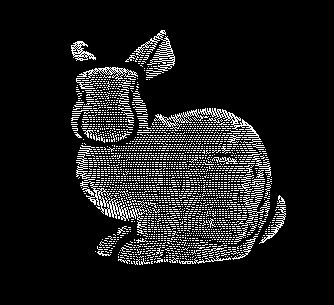
\includegraphics[width=7cm]{bunny-facing-front}
\centering
\caption{The Bunny is facing forward}
\label{fig:bunny-facing-front}
\end{figure}

\pagebreak
\section{Methods Used and Studied}

Given a Point cloud $ P = P_{1},P_{2},P_{3} ... P_{n} $, and a viewpoint \emph{C} our goal is to determine all of the points that are visible from $C $. To put it another way, for every point $ P_{i} $ in $ P$ we would like to determine if $ P_{i} $ is visible from $ C$. We would like to mark a point $ P_{i} $ visible if and only if the point $ P_{i} $ is visible from $ C$.

\subsection{Hidden Point Removal Operator}
Katz et al. \cite{Katz07} introduced an operator called the Hidden Point Removal operator that can be used to determine all of the points that are visible from $C$. The operator consists of two steps:

\begin{enumerate}
\item Spherical inversion
\item Convex hull construction
\end{enumerate}

During spherical inversion we associate the points with a co-ordinate system where the viewpoint $C$ is at the origin. We then map every point $ P_{i} $ along the ray from $ C $ to $ P_{i} $ such that this mapping is monotonically decreasing in the norm ($ || P_{i} ||$). Once we perform the spherical inversion, we compute a convex hull of the transformed set of points $ union $ $ C$, the viewpoint. It is important to note that simply calculating the line of sight from the viewpoint $C$ to the point $ P_{i} $ will always mark the point as visible, except in some degenerate cases. 

What this operator is doing is a simple reduction of the problem of visibility to the problem of convex hull construction. This is because all we are doing is a simple transformation of the points and then computing the convex hull. The complexity of the operator is $ O(nlogn) $ in two and three dimensions and can be extended into higher dimensions. The complexity of the operator is asymptotically similar to that of a convex hull construction, that is $ O(nlogn) $ in two and three dimensions.

\subsection{Spherical inversion}
Consider a D-dimensional sphere with radius $ R $, centered at the origin $ C $, and includes all points in P. Spherical flipping reflects a point $ P_{i} E P $ with respect to the sphere by applying the following equation: 

\begin{equation}
\label{eq:2}
f(P_{i}) = P_{i} + 2 (R - ||P_{i}||) \dfrac{P_{i}}{||P_{i}|} = \widehat{P_{i}}
\end{equation}

Spherical inversion is taking a point internal to some bounding sphere and projecting every point internal to the sphere to its image which is external to the using equation \ref{eq:2}. Spherical inversion reflects every point $ P_{i} $ internal to the sphere along the ray from $ C $ to $ P_{i} $ to its image outside the sphere, as shown in figure \ref{fig:spherical-inversion-1}. 

\begin{figure}[h]
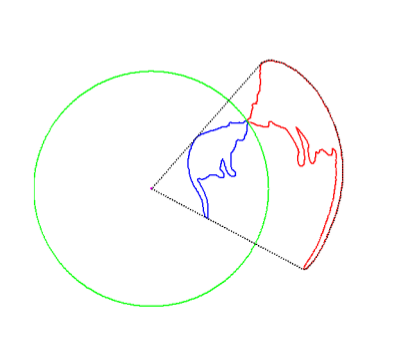
\includegraphics[width=7cm]{spherical-inversion-1}
\centering
\caption{Spherical flipping, shown in red, of a 2D curve, shown in blue, using a sphere, shown in green}
\label{fig:spherical-inversion-1}
\end{figure}

Spherical inversion is taking the blue curve, which is constrained to be bounded in some green circle, which is centered at the origin, or the viewpoint $C$ in our case, and it maps the curve to its image that you see in red, which is the result of the spherical inversion.

\subsection{Convex Hull Construction}
From the spherical flipping above, we have a new point cloud that can be denoted as:
\begin{equation}
\label{eq:3}
\widehat{P} = \hat{P_{1}},\hat{P_{2}},\hat{P_{3}} ... \hat{P_{n}}
\end{equation}

The second, and the final step in our Hidden Point Removal operator is to construct the  convex hull of the new point cloud $\widehat{P} $ union $C$, i.e:

\begin{equation}
C_{hull} = \widehat{P} \cup C
\end{equation}

The points that lie on the convex hull $C_{hull}$ in the equation above  are the points that are visible form $ C $. Figure \ref{fig:spherical-inversion-2} shows projection of the convex hull of the sphere in \ref{fig:spherical-inversion-1}.

\begin{figure}[h]
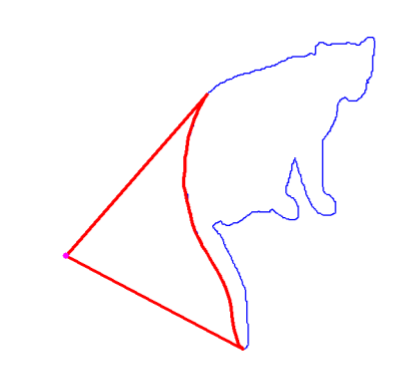
\includegraphics[width=7cm]{spherical-inversion-2}
\centering
\caption{Projection of the convex hull}
\label{fig:spherical-inversion-2}
\end{figure}\textbf{•}

\subsection{The data}

The initial plan was to use data obtained from the \textit{Velodyne HDL-64E LIDAR} scanner by the Motion and Shape Computing (MASC) Group at George Mason University to investigate the visibility of point clouds. While the Point Cloud Library (PCL) \cite{pcl} provides capabilities to read and replay/visualize such data, it became clear that determining visibility of a moving point cloud is beyond the scope of this project. We would need more complex data structures such as kinetic data structures to handle the moving point cloud. 

The data used in the scope of this project are all static models, such as the bunny from Stanford 3D Scanning Repository. The statue of Michelangelo's David was obtained form the PCL's data repository. 

\subsection{The implementation}

Katz et al. \cite{Katz07} made the matlab code for this operator publicly available.
\begin{lstlisting}[language=matlab, caption=Matlab code]
function visiblePtInds=HPR(p,C,param)
	dim=size(p,2);
	numPts=size(p,1);
	% Move the points s.t. C is the origin
	p=p-repmat(C,[numPts 1]);
	% Calculate ||p||
	normp=sqrt(dot(p,p,2));
	% Sphere radius
	R=repmat(max(normp)*(10ˆparam),[numPts 1]);
	%Spherical flipping
	P=p+2*repmat(R-normp,[1 dim]).*p./repmat(normp,[1 dim]);
	%convex hull
	visiblePtInds=unique(convhulln([P;zeros(1,dim)]));
	visiblePtInds(visiblePtInds==numPts+1)=[];
\end{lstlisting}

The goal was to implement this operator in C++ so that it can be used with the Point Cloud Library (PCL) for visualization and various other features that PCL provides. As such, the Hidden Point Operator (HPR) was implemented using PCL and various other libraries, such as Qt5, and VTK, in C++. The program  takes as an input a point cloud in \textit{PCD} or \textit{PLY} format. Figure \ref{fig:point_cloud_library_with_HPR} shows the program with a split window showing the original point cloud and the visibility cloud.

\begin{figure}[h]
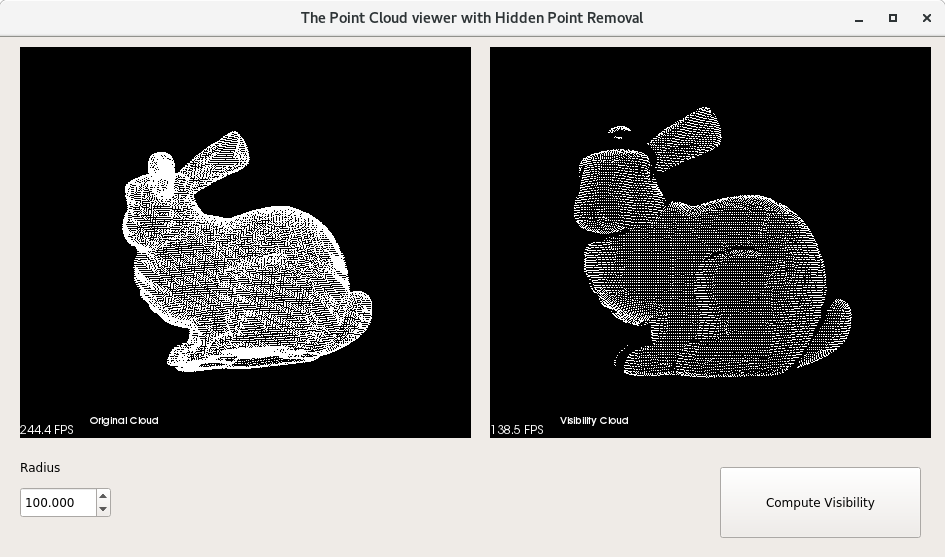
\includegraphics[width=12cm]{point_cloud_library_with_HPR}
\centering
\caption{The Point Cloud viewer with Hidden Point Removal}
\label{fig:point_cloud_library_with_HPR}
\end{figure}

This project will be made publicly available at: https://github.com/pdhimal1/HPR.git

\section{Results/Findings}



\section{Conclusion}


\bibliographystyle{plain}
\bibliography{report}

\listoffigures

\lstlistoflistings


%end of the document
\end{document}


